
\section{Document Access Permission Control}
\label{s-accr}
\subsection{Access Control Policy Configuration}
Since a user requesting access to the storage system for upload/download identifies him/herself with his/her blockchain address, for a solely blockchain-based access authorization, the storage integration gateway should be able to somehow relate a user's blockchain address to the properties of document bearer smart contract. Ideally, the required relation should be defined in the said bearer contract. To provide a generic solution for expressing relationships between contracts and users that covers most scenarios, we treat each document bearer contract as a part of one or more rooted contract relationship hierarchies. Then we provide a path expression language to indicate what contracts reachable from the document bearer contract through different paths contain information about users having some form of access to the underlying document or the storage allocation dedicated for it.     

To understand this concept, consider the scenario where the storage capacity is used to support a blockchain application for crowd-funded real-estate asset developments where investors receive ownership rights on parts of the assets. The asset developer receives the profit for an asset development. However, the actual development work is conducted through a series of activities assigned to sub-contractors. Further, some regulatory agency is tagged with each asset development project by the local branch of the ministry of land for overseeing purposes. Finally, the application allows an investor to trade his/her share on the asset for profit. Then a contract relationship hierarchy for this description can be as illustrated in Figure~\ref{fig-2}. In this description, the root of the relationship is the {\it Project} contract.

\begin{figure}[h]
\centering
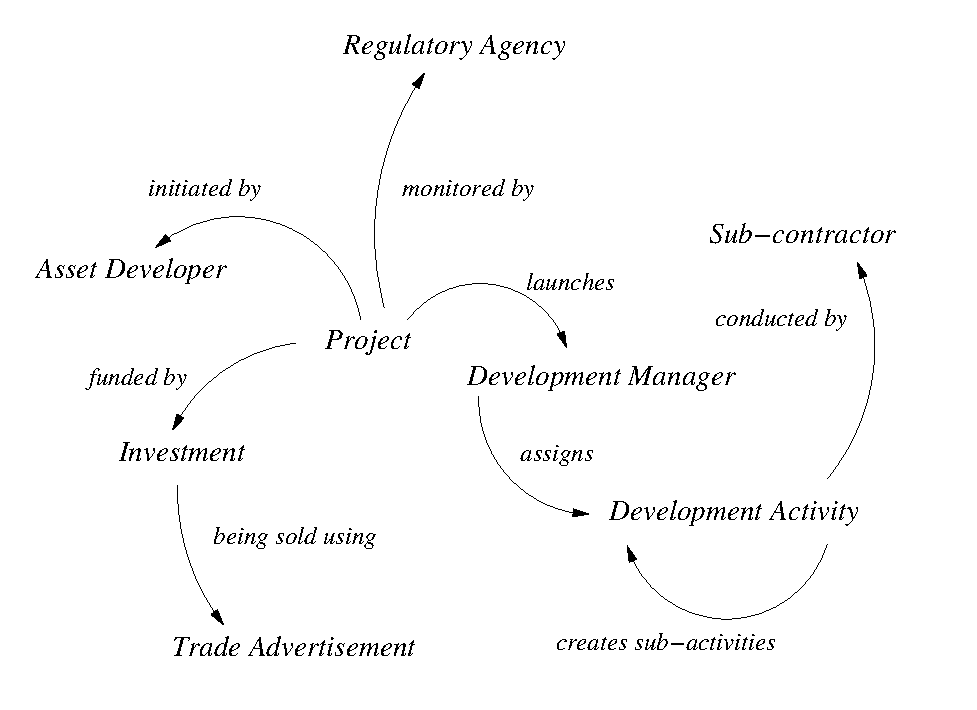
\includegraphics[width=0.48\textwidth]{access-req-example}                    
\caption{An example smart contract relationship hierarchy}\label{fig-2}
\end{figure}
Now if the blockchain application requires that an asset developer can download ``business profile" documents of only those sub-contractors who contributed to his/her asset development projects, this requirement can be expressed in the sub-contractors' smart contracts as a path connecting properties of intermediate contracts and ultimately leading to the asset-developer. The advantage of using path expressions instead of using blockchain addresses of corresponding entities directly is that if their relationship is broken due to some property update in the intermediate contracts, the document access permission is automatically revoked. Likewise, new users are granted access to documents automatically     as new relationships are established in the blockchain.

To make this scheme work in the current Ethereum smart contract specification, we only need that each smart contract belongs to some predefined contract template and bears with it a template type identifier and a method to list all its properties. If there was a mechanism to search the property names of an arbitrary smart contract deployed in the blockchain, the template typing would not be required. Anyway, we believe this is not a difficult requirement to satisfy.   
   
\begin{figure}[t!]
\scriptsize
%\footnotesize
\begin{bnf*}
\bnfprod{permission} {\bnfpn{docperms} \bnfor \bnfes}\\
\bnfprod{docperms}{\bnfpn{docperm} \bnfor \bnfpn{docperm} \bnfsp \bnfts{;} \bnfsp \bnfpn{docperms}}\\
\bnfprod{docperm}{\bnfpn{doctype} \bnfsp \bnfpn{userperms}}\\
\bnfprod{userperms}{\bnfpn{userperm} \bnfor \bnfpn{userperm} \bnfsp \bnfts{AND} \bnfsp \bnfpn{userperms}}\\
\bnfprod{userperm}{\bnfts{[} \bnfsp \bnfpn{permbits} \bnfsp \bnfts{]} \bnfsp \bnfpn{permexpr}}\\
\bnfprod{permexpr}{\bnfpn{localexpr} \bnfor \bnfpn{remoteexpr}}\\
\bnfprod{doctype}{\bnfpn{attrname} \bnfsp \bnfts{:} \bnfsp \bnfpn{attrmult} \bnfsp \bnfts{--}}\\
\bnfprod{permbits}{\bnfts{r-} \bnfor \bnfts{-w} \bnfor \bnfts{rw}}\\
\bnfprod{localexpr}{\bnfts{(} \bnfsp \bnfpn{attrname} \bnfsp \bnfts{:} \bnfsp \bnfpn{attrmult} \bnfsp \bnfts{)}}\\
\bnfprod{remoteexpr}{\bnfpn{acclink} \bnfsp \bnfts{/} \bnfsp \bnfpn{srclink} \bnfsp \bnfts{/} \bnfsp \bnfpn{overlap}}\\
\bnfprod{acclink}{\bnfts{accessor} \bnfsp \bnfts{(} \bnfpn{attrmult} \bnfsp \bnfts{)} \bnfsp \bnfts{[} \bnfpn{pathdirection} \bnfsp \bnfts{]} \bnfsp \bnfts{=} \bnfpn{path} \bnfsp \bnfts{=} \bnfsp \bnfts{root}}\\
\bnfprod{srclink}{\bnfts{this} \bnfsp \bnfts{=} \bnfsp \bnfpn{path} \bnfsp \bnfts{=} \bnfsp \bnfts{root}}\\
\bnfprod{overlap}{\bnfts{none} \bnfor \bnfts{substr}}\\
\bnfprod{pathdirection}{\bnfts{F} \bnfor \bnfts{R}}\\
\bnfprod{path}{\bnfpn{edge} \bnfor \bnfpn{edge} \bnfsp \bnfts{--} \bnfsp \bnfpn{path}}\\
\bnfprod{edge}{\bnfpn{linkerprop} \bnfsp \bnfts{:} \bnfsp \bnfpn{contracttype} \bnfsp\bnfpn{occurrences}}\\
\bnfprod{attrname}{\bnfpn{string}}\\
\bnfprod{attrmult}{\bnfts{single} \bnfor \bnfts{array}}\\
\bnfprod{linkerprop}{\bnfpn{string}}\\
\bnfprod{contracttype}{\bnfpn{string}}\\
\bnfprod{occurrences}{\bnfes \bnfor \bnfts{[*]}}
\end{bnf*}
\normalsize
\caption{Permission Expression Grammar}
\label{grammar}
\end{figure}

Figure~\ref{grammar} describes the grammar for permission policy configuration for a document bearer smart contract. The grammar requires that access permissions are specified per document type and individually for each approved user category. There are three components of each permission expression that grants a specific kind of users an specific kind of access to a specific document of a specific type of smart contract:
\begin{enumerate}
\item Source Linkage: a path description that tells how the root of the contract relationship hierarchy can be reached from the document bearer contract.
\item Accessor Linkage: another path description that tells how the root of the contract relationship hierarchy can be reached from the contract holding the user address.
\item Path Intersection Requirement: a specification that tells to what extent the source and accessor linkages should overlap to grant the user access to the document.
\end{enumerate}

For example, assume in the contract relationship hierarchy of Figure~\ref{fig-2}, the {\it investor} of any {\it Investment} contract, the {\it assigner} of an ancestor {\it DevActivity} contract, and any of the {\it representatives} of the {\it RegulatoryAgency} contract can view the {\it license} document of the {\it Subcontractor} contract corresponding to the {\it assignee} of a {\it DevActivity} of the underlying project. Meanwhile, only the {\it owner} of the {Subcontractor} contract can both read and replace (i.e., write) the {\it license} document in the external storage. Then the permission configuration for the {\it license} document should be as described in Listing~\ref{perm-ex}:
\lstset{caption=Example access permission configuration, label=perm-ex}
\lstinputlisting{permission-example.txt}
Our strategy for specifying the access permissions using contract relationship path expressions is a middle ground between access control list (ACL) and role based access control (RBAC) that are typically being used in file systems \cite{Barkley:1997:CSR:266741.266769}. Like RBAC, users gain access to resources because they held specific roles due to their association with specific smart contracts. Unlike generic roles in RBAC, however, roles in our case are indirectly bound to specific resources through some relationship graphs.       

\subsection{Access Control Policy Enforcement}
A storage integration gateway does not need to understand specific smart contract relationship hierarchies to enforce access control rules specified in the permission expressions of various smart contracts. It only requires that the blockchain network notifies it whenever a smart contract is deployed and contracts emit properly formatted events\footnote{An event should contain the addresses of the two contracts whose direct association has been affected by the blockchain transaction, their template type names, and the nature of the update.} in the blockchain audit log in response to blockchain transactions that may affect any source or accessor linkages.\footnote{If we consider a smart contract relationship hierarchy as a directed graph, all relationships may not be traceable from the leaf to the root of the hierarchy. Some relationships may go backward from the root to the leave. Regardless, the events on the audit log should be formatted to support a uniform traversal strategy from the leave to the root.}

The gateway monitors these events and derives a document permission database by combining event data and gateway's path expression related query results. This database is like a dynamic ACL database that is automatically being updated in response to new blockchain events. Figure~\ref{fig:perm-ERD} depicts a high level entity relationship diagram of the gateway database.
\begin{figure}[h]
\centering
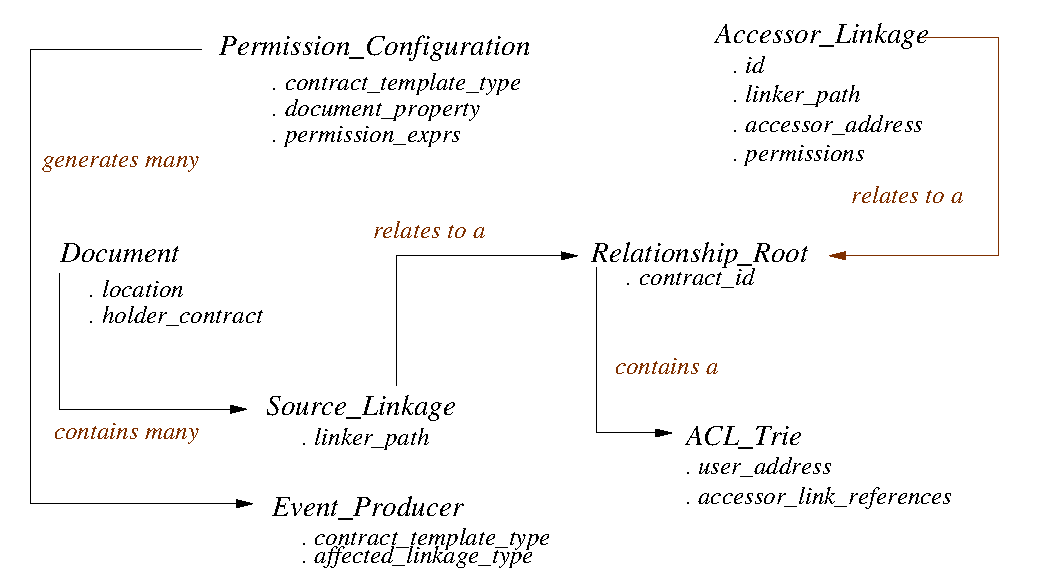
\includegraphics[width=0.48\textwidth]{permission-db}                    
\caption{Entity Relationship Diagram of the Access Permission Database}\label{fig:perm-ERD}
\end{figure}
As new smart contracts are being deployed in the blockchain network, the gateway updates contracts' template related information in local database to determine if a contract of this type can affect any document access permission through some source and accessor linkages. The gateway also determines if this type of contract can be a root of any contract relationship hierarchy. For each contract that is a root of a relationship hierarchy, the gateway creates an ACL holding Merkle tree \cite{6233691} that contains the user addresses that are the endpoints of various accessor linkages originated from the root.

If a document is uploaded or an event is published about a change in any property that contributes an edge to the document's paths to various relationship roots, new source linkages are being computed and stored in the database. At the same time, invalidated source linkages are being eliminated. Similarly, if any smart contract property that contributes an edge to users' accessor path to various relationship roots, valid accessor linkages are being recomputed. In addition, the ACL tree entries of the affected users are also being updated.

When a user requests the gateway to undertake an upload/download protocol with the user, the gateway receives the underlying document bearing smart contract's address, the attribute of the smart contract the document refers to, and the user address. Since in case of an upload, the user must be associated with the document bearing smart contract directly, the gateway merely checks the smart contract template description to determine what query to issue in the smart contract to search for the user. If the requesting user is found registered as a valid uploader, the upload protocol initiates. Once upload is done, blockchain audit log is traversed to determine new source linkages for that document to existing contract relationship roots. These linkages are then inserted in the gateway database. If the new document replaces some document uploaded earlier then only the location related metadata need to be updated in the gateway database to point to the new document.       

If the user requests for a document download session, the gateway first identifies the ACL trees correspond to smart contract relationship roots reachable by traversing the source linkages of the document. Then it checks if the user's address is in any of those trees. Then it retrieves all accessor linkages ending at the user address in various trees. Finally, related document source and accessor linkages are compared to decide if they can be combined satisfying any read permission configuration for the document. If a combination attempt succeeds then the user is granted access. If the authorization process fails in any step then the user's request is denied.          
        